% !Mode:: "TeX:UTF-8"%確保文檔utf-8編碼
\documentclass[tikz,border=2pt]{standalone}

\begin{document}
\begin{tikzpicture}
%draw the axes
\draw[->] (0,0,0) -- (3,0,0) node[anchor=west]{$x$};
\draw[->] (0,0,0) -- (0,3,0) node[anchor=west]{$y$};
\draw[->] (0,0,0) -- (0,0,3) node[anchor=west]{$z$};
%draw the top and bottom of the cube
\draw (0,0,0) -- (0,2,0) -- (2,2,0) -- (2,0,0) -- cycle;
\draw[] (0,0,2) -- (0,2,2) -- (2,2,2) -- (2,0,2) -- cycle;
	
%draw the edges of the cube
\draw[] (0,0,0) -- (0,0,2);
\draw[] (0,2,0) -- (0,2,2);
\draw[] (2,0,0) -- (2,0,2);
\draw (2,2,0) -- (2,2,2);
\end{tikzpicture}


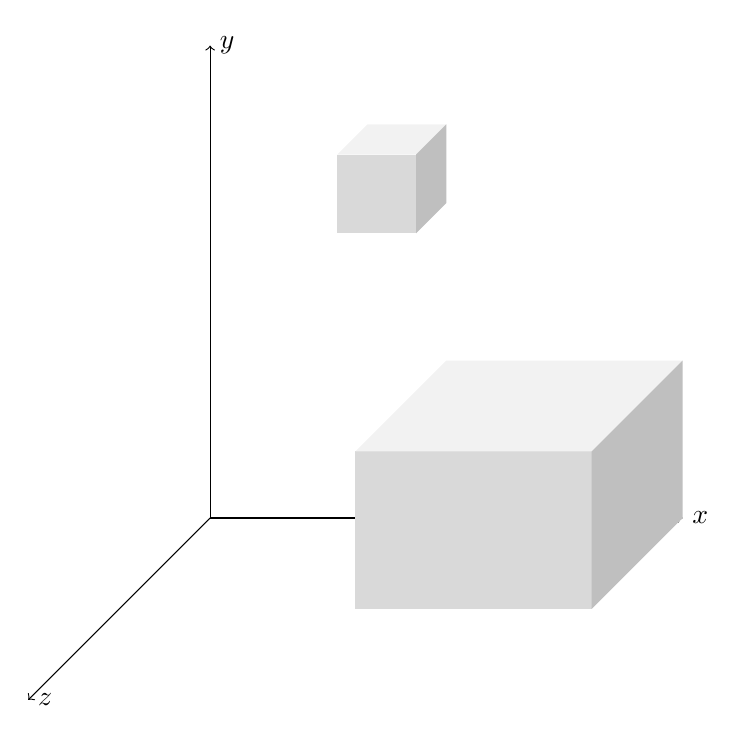
\begin{tikzpicture}
%draw the axes
\draw[->] (0,0,0) -- (6,0,0) node[anchor=west]{$x$};
\draw[->] (0,0,0) -- (0,6,0) node[anchor=west]{$y$};
\draw[->] (0,0,0) -- (0,0,6) node[anchor=west]{$z$};

\newcommand\cube[4][]{
\begin{scope}[#1]%长方体2
\def\x{#2}
\def\y{#3}
\def\z{#4}
\fill[gray!30] (0,0,\z) -- (\x,0,\z) -- (\x,\y,\z) -- (0,\y,\z);
\fill[gray!10] (0,\y,\z)-- (0,\y,0) -- (\x,\y,0) -- (\x,\y,\z)  ;
\fill[gray!50] (\x,0,\z) -- (\x,0,0) -- (\x,\y,0) --(\x,\y,\z);
\end{scope}}


\cube[xshift=3cm]{3}{2}{3}

\cube[yshift=4cm,xshift=2cm]{1}{1}{1}


\end{tikzpicture}


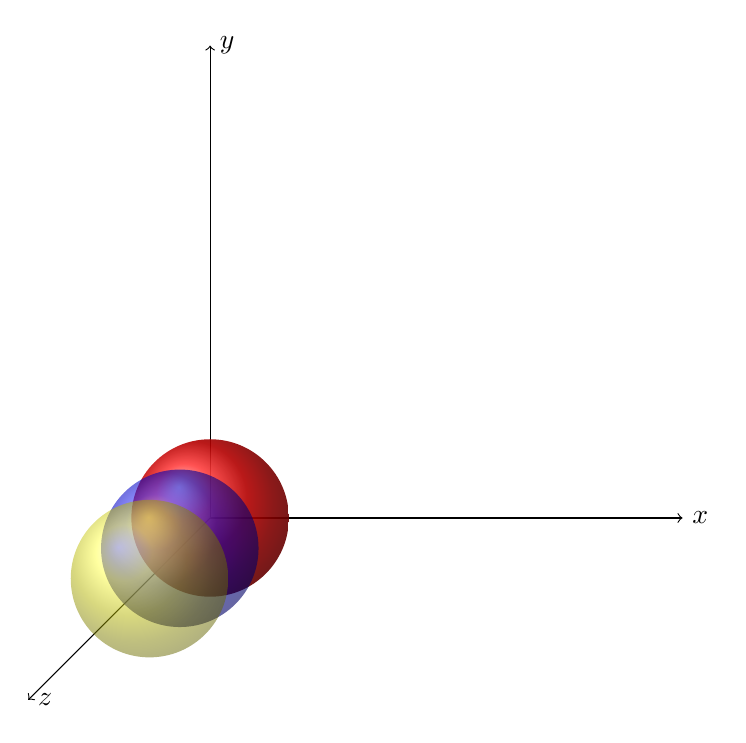
\begin{tikzpicture}
%draw the axes
\draw[->] (0,0,0) -- (6,0,0) node[anchor=west]{$x$};
\draw[->] (0,0,0) -- (0,6,0) node[anchor=west]{$y$};
\draw[->] (0,0,0) -- (0,0,6) node[anchor=west]{$z$};

\shade[ball color=red,opacity=0.9] (0,0,0) circle (1);

\shade[ball color=blue,opacity=0.6] (0,0,1) circle (1);

\shade[ball color=yellow,opacity=0.5] (0,0,2) circle (1);
\end{tikzpicture}

\end{document}